\documentclass[12pt,a4paper]{article}

\usepackage{geometry}
\geometry{
    left=2cm, 
    right=2cm,
    top=3cm,  
    bottom=2cm
}

\usepackage[spanish,english]{babel}
\usepackage[utf8]{inputenc}
\usepackage{amsmath}

\usepackage{graphicx}
\usepackage{wrapfig}

\usepackage{booktabs}
\usepackage{enumitem}
\usepackage{xcolor}


\usepackage{csquotes}
\usepackage{hyperref}
\usepackage[style=ieee]{biblatex}
\addbibresource{referencias.bib}

\usepackage{setspace}
\setstretch{1.5}
\setlength{\parindent}{0pt}

\begin{document}
    \begin{titlepage}
        \begin{minipage}[c]{0.1\textwidth}
            
\includegraphics[width=\textwidth]{Resources/logo_unam.jpg}
        \end{minipage}
        \begin{minipage}{0.8\textwidth}
            \centering
            {\Large\textbf{Universidad Nacional Autónoma de México}\\}
            {\large\textbf{Escuela Nacional de Estudios Superiores\\\underline{Unidad Morelia}}}
        \end{minipage}
        \begin{minipage}[c]{0.1\textwidth}
            
\includegraphics[width=\textwidth]{Resources/logo_enes.jpg}
        \end{minipage}
        \vspace{3cm}

        \centering
        {\large{Reporte Final\\}}
        {\Large\textbf{Análisis de Valores Nutricionales por Tipo de Dieta}}
        \vspace{2cm}

        {{PRESENTA:\\}}
        {\large\textbf{Alexis Uriel Aguilar Uribe}}
        \vspace{1cm} 

        {{PROFESORES:\\}}
        {\large\textbf{Dra.\ María Del Río Francos}}\\
        {\large\textbf{Dr.\ César Andrés Torres Miranda}}
        \vspace{2cm}

        {{GRADO\\}}
        {\large\textbf{Licenciatura en Tecnologías para la Información en Ciencias}}
        \vspace{2cm}

        \flushleft{
        {\textbf{Asignatura:\ }Estadística Descriptiva e Inferencial}
        \vspace{2cm}}

        \flushright{
        {\textbf{A:\ }\underline{21 de Mayo del 2025}}}
        \vfill
    \end{titlepage}

\newpage

\tableofcontents

\newpage

\section{Introducción}

    Este trabajo tiene como fin de exponer el proceso llevado a cabo para 
    realizar el análisis estadístico de los valores nutricionales (macronutrientes) 
    que aportan las dietas: \emph{DASH} (Dietary Approaches to Stop Hypertension), 
    \emph{keto}, \emph{mediterránea}, \emph{paleo} (paleolítica) y \emph{vegana}.\\

    Siendo el principal enfoque el responder si hay una diferencia nutricional 
    significativa entre las diferentes dietas. En decir, hacer uso de 
    técnicas de estadística descriptiva e inferencial para probar si existe 
    una diferencia en los aportes nutricionales entre las distintas dietas que 
    están siendo estudiadas. La anterior prueba se basa en recetas de diferentes 
    cocinas a nivel mundial.

    El propósito final del presenta trabajo es el de crear un modelo estadístico 
    capaz de categorizar la dieta a la que pertenece una receta en base a los 
    macronutrientes (carbohidratos, proteínas y grasas) que aporta.

\section{Objetivos Generales}

    Para la realización de lo anterior expuesto, se puntualizan los objetivos del 
    proyecto:
    \begin{itemize}
        \item Realizar análisis estadístico de los macronutrientes en las diferentes. 
        Para una caracterización de los aportes nutricionales.
        \item Conjeturar y probar hipótesis sobre los aportes nutricionales de 
        cada dieta en base a su comportamiento estadístico y definición.
        \item Probar si existe una diferencia significativa en los aportes 
        nutricionales entre las diferentes dietas con el fin de crear un 
        modelo clasificar de recetas basado en sus aportes nutricionales.
    \end{itemize}

\newpage

\section{Marco Teórico}
    
    La dieta es uno de los principales factores de riesgo de las enfermedades 
    crónicas, y las enfermedades sensibles a la dieta contribuyen en gran medida 
    a los costes sanitarios mundiales. Se han propuesto literalmente miles de 
    \emph{dietas}, que pueden describirse en términos generales como basadas en 
    creencias, en alimentos específicos o en nutrientes; centradas en la 
    pérdida de peso o en el aumento de peso (muscular); dietas de desintoxicación 
    (detox) y dietas diseñadas por razones médicas específicas.\cite{marvastipopular} \\

    Las \emph{dietas de moda} son dietas populares durante un tiempo sin basarse 
    necesariamente en una recomendación dietética estándar. A menudo promueven 
    una pérdida de peso irracionalmente rápida o afirmaciones de salud sin 
    sentido, y se anuncian como dietas que requieren poco esfuerzo por parte de 
    quien las sigue. La promesa de ganancias fáciles, combinada con la presión 
    social para lograr un determinado tipo de cuerpo, puede dejar al público 
    susceptible a afirmaciones infundadas o exageradas.\cite{marvastipopular} \\

    Las dietas estudiadas desde una perspectiva estadística en el presente 
    trabajo, son englobadas en las \emph{dietas de moda}, que a veces son referidas 
    como \emph{dietas sin evidencia científica}. Siendo  la dieta DASH la única 
    que cuenta con algún tipo de fundamento.

    \subsection{DASH (Dietary Approaches to Stop Hypertension)}

        \cite{marvastipopular} La dieta DASH (Enfoques Dietéticos para Detener la 
        Hipertensión) es un patrón dietético diseñado específicamente para ayudar 
        a reducir la presión arterial y promover la salud general del corazón. Hace 
        hincapié en el consumo de una variedad de alimentos ricos en nutrientes, 
        como frutas, verduras, cereales integrales, proteínas magras y productos 
        lácteos bajos en grasa, y en la limitación de la ingesta de sodio, grasas 
        saturadas y azúcares añadidos. 

    \subsection{Dieta Keto}

        \cite{marvastipopular} Una dieta baja en hidratos de carbono (baja en 
        carbohidratos) es un patrón alimentario que restringe la ingesta de 
        carbohidratos, sustituyéndolos normalmente por mayores cantidades de 
        proteínas y grasas. La dieta cetogénica es una forma de dieta baja en 
        carbohidratos con un alto contenido en grasas en relación con la ingesta 
        de proteínas y carbohidratos.\\

        El objetivo de la dieta cetogénica es inducir la cetosis, un estado 
        metabólico que se produce cuando el cuerpo quema grasa para obtener 
        energía en lugar de glucosa, lo que induce la pérdida de peso.

    \subsection{Dieta Mediterránea}

        \cite{marvastipopular} La dieta mediterránea es un patrón alimentario 
        inspirado en los hábitos alimenticios tradicionales de los países 
        situados a orillas del mar Mediterráneo. Se caracteriza por un alto consumo 
        de frutas, verduras, cereales integrales, legumbres, frutos secos y 
        aceite de oliva; un consumo moderado de pescado y aves; y un bajo 
        consumo de carnes rojas, alimentos procesados y dulces.\\

    \subsection{Dieta Paleo (Paleolítica)}

        \cite{marvastipopular} La dieta paleo, también conocida como dieta 
        paleolítica o dieta del hombre de las cavernas, es un enfoque 
        dietético que pretende imitar los hábitos alimentarios de nuestros 
        antiguos antepasados del Paleolítico. \\

        Hace hincapié en el consumo de alimentos integrales y no procesados 
        que habrían estado al alcance de los primeros humanos, como carnes magras, 
        pescado, frutas, verduras, frutos secos y semillas, y excluye los cereales, 
        las legumbres, los productos lácteos, los alimentos procesados y los 
        azúcares añadidos.

    \subsection{Dieta Vegana}

        \cite{marvastipopular} La dieta vegana es un patrón dietético basado en 
        plantas que excluye el consumo de todos los productos de origen animal. Se 
        centra en el consumo de una variedad de alimentos de origen vegetal, como 
        frutas, verduras, cereales legumbres, frutos secos y semillas.\\

        Es importante señalar que, aunque las dietas veganas pueden ser 
        nutricionalmente adecuadas, debe prestarse atención a garantizar una 
        ingesta suficiente de nutrientes esenciales como proteínas, hierro, 
        calcio, vitamina B12 y ácidos grasos omega-3.

\newpage

\section{Presentación de los Datos}

    \subsection{Fuente de Datos}

        El conjunto de datos con el que se está trabajando para este trabajo 
        se encuentra en \cite{dataset_macronutrients}, publicado por la comunidad 
        de Kaggle. Los datos consisten de un conjunto de recetas de diferentes 
        dietas y cocinas, además incluye información de los macronutrientes que 
        aporta cada receta.\\

        \cite{dataset_macronutrients} Aunque en la descripción ni en los metadatos del conjunto de datos se 
        haga mención de las fuentes explícitas de los datos ni el objetivo de 
        esta extracción, sí cuenta con una sección de cómo usar el conjunto de 
        datos, ideas de investigación y reconocimientos.\\

        De los apartados de cómo usar el conjunto de datos e ideas de investigación, 
        se encuentra una idea, implícita, de la información que se quería estudiar. 
        La principal información de interés se vuelve que es: el crear planes 
        alimenticios saludables, ya sea usando las recetas proporcionadas o creando 
        unas nuevas basadas en una dieta y cocina, y el estudiar la relación entre 
        dieta y salud.\\

        Del apartado de reconocimientos, se concluye que las recetas fueron 
        proporcionadas por diferentes creadores de las mismas y demás contribuidores 
        al conjunto de datos. 

    \subsection{Interés del Estudio}

        Se consultó \cite{marvastipopular} en sus 
        capítulos 4 y 8, de donde se proporciona un mejor entendimiento de la 
        importancia de los macronutrientes y una descripción general de las 
        dietas en este trabajo, resultando interesante que en cada dieta se 
        consumen diferentes alimentos y productos con ciertas características 
        para ya sea respetar alguna creencia, fundamento o cuota de macronutrientes. 
        De esto último, proporciona un indicio de que existe una diferencia entre 
        las dietas a nivel de sus aportes nutricionales, por lo tanto, lo que se 
        quiere realizar es probar esta diferencia de manera significativa haciendo 
        uso de la estadística.

    \subsection{Variables del Conjunto de Datos}

        El conjunto de datos consta de las siguientes variables. Se menciona su 
        nombre, el tipo de variable y sus valores (en total y únicos):

        \begin{center}
            \begin{tabular}{| c | c | c | c | c |}
                \toprule
                Variable & Nombre & Tipo & Cantidad de Datos & Valores Únicos\\
                \midrule
                1 & Diet\_type & Cualitativa Nominal & 7806 & 5 \\
                2 & Recipe\_name & Cualitativa Nominal & 7806 & 7062\\
                3 & Cuisine\_type & Cualitativa Nominal & 7806 & 19\\
                4 & Protein(g) & Cuantitativa Continua & 7806 & 6060\\
                5 & Carbs(g) & Cuantitativa Continua & 7806 & 6618\\
                6 & Fat(g) & Cuantitativa Continua & 7806 & 6322\\
                \bottomrule
            \end{tabular}
        \end{center}

        La variable \emph{Recipe\_Name} no es relevante para este trabajo pero figura 
        dentro del dataset. Se hace mención que el conjunto de datos no presenta 
        valores faltantes.

    \subsection{Ejemplo de Registros en el Conjunto de Datos}

        Para ejemplificar como luce el conjunto de datos, se presente 
        una instancia de cada tipo de dieta:

        \begin{center}

            \begin{tabular}{| c | c | c |}
                \toprule
                \textbf{Diet\_type} & \textbf{Recipe\_name} & \textbf{Cuisine\_type} \\
                \midrule
                \small{dash}          & \small{Old Fashioned                     }& \small{world} \\
                \small{keto}          & \small{Keto Egg Drop Soup                }& \small{chinese} \\
                \small{mediterranean} & \small{Mediterranean Mix                 }& \small{mediterranean} \\
                \small{paleo}         & \small{Easy Paleo Herb Gravy recipes     }& \small{french} \\
                \small{vegan}         & \small{Braised Green Beans with Tomatoes }& \small{mediterranean} \\
                \bottomrule
            \end{tabular}

        \end{center}

        \begin{center}

            \begin{tabular}{| c | c | c |}
                \toprule
                \textbf{Protein(g)} & \textbf{Carbs(g)} & \textbf{Fat(g)} \\
                \midrule
                 \small{0.12} &  \small{9.66} &  \small{0.02} \\
                \small{21.31} &  \small{9.11} & \small{60.88} \\
                 \small{8.11} &  \small{9.59} & \small{14.64} \\
                \small{23.56} & \small{39.05} & \small{42.25} \\
                \small{17.49} & \small{77.86} & \small{70.20} \\
                \bottomrule
            \end{tabular}

        \end{center}

\newpage

\section{Estadística Descriptiva}

    Debido a que cada receta puede aportar una amplia variedad de valores 
    en sus macronutrientes, esto podría dificultar la comparación entre 
    los aportes nutricionales de las dietas. Por ello, para reducir este 
    sesgo, se aplico una normalización a los valores, es decir, 
    los macronutrientes de cada receta se dividió por el total de macronutrientes 
    que aportaba la receta, para así manejar los aportes proporcionales de 
    cada macronutriente en cada una de las recetas. De aquí en adelante, cuando 
    se mencionan los aportes nutricionales o por macronutriente de una receta, 
    siempre se hace referencia a estos aportes proporcionales respecto al total de 
    macronutrientes en una receta. 

    \subsection{Transformación de Datos}

        Debido a que el rango de los valores que pueden tomar los macronutrientes 
        es un rango amplio y que, además, podría dificultar la comparativa a lo largo 
        de las diferentes dietas en sus aportes nutricionales, se decidión que los 
        valores en los macronutrientes sean transformados para trabajar con aportes 
        relativos al total de macronutrientes de cada receta o, equivalentemente, los 
        aportes absolutos de los macronutrientes se normalizaron con la norma $L_1$.\\

        De la anterior transformación, se creó una nuevo atributo que representa el 
        total de macronutrientes que son aportados por cada receta y el rango de los 
        valores que pueden tomar los macronutrientes es $[0,1]$ donde se verifica que 
        la suma de los tres valores (a lo largo de los macronutrientes) sea siempre $1$. 
        Este último punto va a permite generar una representación visual de la distribución 
        de las recetas en el plano y servirá para determinar las teóricas distribuciones de 
        los macronutrientes, en específico los parámetros de la distribución beta que mejor 
        se ajusta a la distribución de cada macronutriente y dieta; esto permite caracterizar 
        las disitrbuciones desde una perspectiva teórico que será relevante para responder 
        la pregunta central de trabajo.

        Para el conjunto de datos resultante de la transformación también se les renombraron 
        algunos de sus atributos pero que siguen representando o significando el mismo concepto.

        \begin{center}

            \begin{tabular}{| c | c | c |}
                \toprule
                \textbf{Diet\_type} & \textbf{Recipe\_name} & \textbf{Cuisine\_type} \\
                \midrule
                \small{dash}          & \small{Old Fashioned                     }& \small{world} \\
                \small{keto}          & \small{Keto Egg Drop Soup                }& \small{chinese} \\
                \small{mediterranean} & \small{Mediterranean Mix                 }& \small{mediterranean} \\
                \small{paleo}         & \small{Easy Paleo Herb Gravy recipes     }& \small{french} \\
                \small{vegan}         & \small{Braised Green Beans with Tomatoes }& \small{mediterranean} \\
                \bottomrule
            \end{tabular}

        \end{center}

        \begin{center}

            \begin{tabular}{| c | c | c | c |}
                \toprule
                \textbf{Protein} & \textbf{Carbs} & \textbf{Fat} & \textbf{Total\_Macronutrients} \\
                \midrule
                \small{0.9857} & \small{0.0122} & \small{0.0020} & \small{  9.80} \\
                \small{0.0997} & \small{0.2334} & \small{0.6668} & \small{ 91.30} \\
                \small{0.2965} & \small{0.2507} & \small{0.4526} & \small{ 32.34} \\
                \small{0.3724} & \small{0.2246} & \small{0.4029} & \small{104.86} \\
                \small{0.4703} & \small{0.1056} & \small{0.4240} & \small{165.55} \\
                \bottomrule
            \end{tabular}

        \end{center}

    \subsection{Descripción de los Valores de las Variables}

        Para el presente trabajo se harán uso de las siguientes variables, se 
        acompañan con una descripción de su significado:

        \begin{itemize}[label=\textbullet]

            \item \textbf{Diet\_type}: Variable que representa el tipo de 
            dieta (DASH, keto, mediterránea, paleo, vegana) a la que 
            pertenece una receta. Con esta variable se va permitir estratificar 
            las recetas y estudiarlas de una manera más granular, es decir, 
            por tipo de dieta para llegar a conformar hipótesis sobre lo qué 
            está pasando en una dieta o entre las diferentes dietas.

            \item \textbf{Cuisine\_type}: Variable que representa a qué (estilo 
            de) cocina o región (mexicana, americana, italiana, entre otras) pertenece una 
            receta. Al usarla va a permitir el comparar cómo son las recetas 
            de una dieta en diferentes regiones, en específico el 
            como se compara la dieta mediterránea en el mediterráneo  
            contra otras regiones geográficas.

            \item \textbf{Protein(g)}: Después de la transformación, representa el 
            porcentaje, respecto al total de macronutrientes, de proteínas que son 
            aportados por una receta. El usar las proteínas va a permitir la 
            comparación entre diferentes dietas, siendo esto el eje central del trabajo

            \item \textbf{Carbs(g)}: Después de la transformación, representa el 
            porcentaje, respecto al total de macronutrientes, de carbohidratos que 
            son aportados por una receta. Siendo otro de los macronutrientes de una 
            comida, se vuelve relevante para la comparación entre recetas y dietas.

            \item \textbf{Fat(g)}: Después de la transformación, representa el 
            porcentaje, respecto al total de macronutrientes, de grasas que son 
            aportados por una receta. Y el último macronutriente, como en los 
            anteriores, se vuelve una variable relevante para la comparación entre dietas.
        \end{itemize}

    \subsection{Medidas de Tendencia Central y Dispersión}
        Realizando el resumen de las medidas, se tiene:

        \begin{center}
            \begin{tabular}{| c | c c c |}
                \toprule
                Medida & Carbs(g) & Protein(g) & Fat(g) \\
                \midrule
                Media               & 0.433471 & 0.234762 & 0.331767 \\
                $Q_1$               & 0.205251 & 0.110188 & 0.184583 \\
                $Q_2$               & 0.432028 & 0.190931 & 0.314359 \\
                $Q_3$               & 0.635058 & 0.338059 & 0.464532 \\
                Desviación Estándar & 0.256032 & 0.163886 & 0.194920 \\
                Mínimo              & 0.000330 & 0.000000 & 0.000000 \\
                Máximo              & 1.000000 & 0.887557 & 0.997940 \\
                Asimetría de Fisher & 0.189556 & 0.922401 & 0.461455 \\
                \bottomrule
            \end{tabular}
        \end{center}

        Debido a que son medidas sobre todos los datos, sin estratificar, 
        se tiene que no hay una referencia de lo que se espera obtener y 
        parte de la información que contienen queda diluida o desvanecida. 
        Esto debido a que las dietas como la vegana es baja en proteínas y 
        la keto en carbohidratos \cite{marvastipopular}, por lo que cualquier 
        suposición no se podría sostener sobre todos las dietas.\\

        Aún así, se reportan bajos valores en proteínas en comparación 
        con los carbohidratos y grasas si se hace uso de la mediana ($Q_2$), 
        dicho así: el cincuenta por ciento de las recetas tienen a lo mucho  
        $19.09\%$ de proteínas, en comparación con el $43.20\%$ de carbohidratos 
        y el $31.43\%$ de grasas. Esto es un indicio de que las recetas, en general, 
        tienden a ser altas en carbohidratos y grasas entre las diferentes dietas y 
        cocinas; mientras que son bajas en proteínas. Este último punto puede ser apoyado si se considera la media de los 
        macronutrientes, que siguen esta tendencia de aportes.\\

        Si se gráfica la distribución de los macronutrientes se tiene que, debido 
        a la asimetría y a la desviación estándar, contienen datos atípicos en proteínas y grasas en una región 
        positiva respecto a la mediana, y esto se relaciona con lo mencionado de que 
        una receta no tiende a un aporte alto de proteínas. Y si se consider el rango 
        intercuartil, se observa que en estos macronutrientes es menor, en comparación, 
        que con el de los carbohidratos, esto muestra como los valores de proteínas y 
        grasas se encuentran concentradas en ciertas regiones en contraste con los posibles 
        valores de los carbohidratos que son más diversos.
        
        \begin{center}
            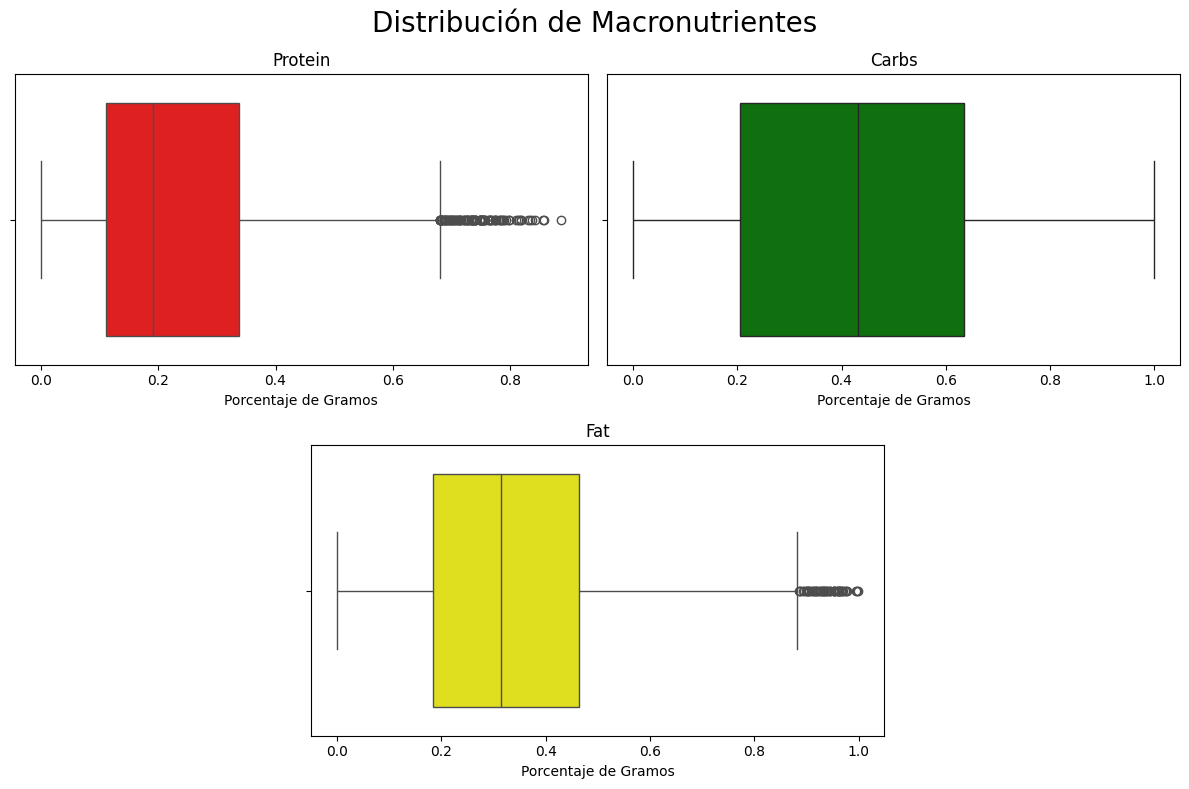
\includegraphics[width=0.75\textwidth]{Resources/2_02_plot_01.png}
        \end{center}

        Debido a que existe la presencia de datos atípicos, lo más adecuado es tratarlos 
        de manera estratificada, por tipo de dieta. Esto debido a que tratarlos de manera 
        general podría evocar que ciertas dietas queden menos representadas en comparación 
        con otras o que incluso se pierda información para consecuentes procesos. Y al 
        tratar los valores atípicos dentro de cada dieta permite reducir el impacto de 
        perder información valiosa y se siga conservando las recetas relevantes para una dieta.

    \subsection{Estratificación de Valores Cuantitativos}

        La variable \emph{Diet\_type} es la principal que se emplea para la 
        estratificación de las recetas, debido a que permite seprarlas 
        según una criterio bien definida, a qué dieta pertenecen. Para cada 
        una de las cinco dietas se presentan los datos tabulados de sus 
        medidas de tendencia central y dispersión junto con su histograma 
        de los valores en sus macronutrientes.\\

        \subsubsection{Dieta DASH}

            Una receta de esta dieta tendrá que, en promedio, el $55\%$ de sus 
            macronutrientes son carbohidratos (provenientes de frutas, vegetales 
            y granos enteros); el $25\%$ son grasas que, por su naturaleza, son 
            saludables; y el $20\%$ son proteínas, las cuáles provienen de carnes margas.\\
            Aunque esta dieta se menciona ser saludable para la salud cardiovascular, 
            no implica que exista un balance o equilibrio en los macronutrientes 
            consumidos por receta.\\

            El cincuenta por ciento de las recetas tienen entre $33\%$ y $76\%$ 
            de carbohidratos en su composición, este fenómeno se puede observar 
            también	en su desviación estándar. Esto implica que los carbohidratos 
            pueden estar en cualquier proporción pero con una tendencia a tener 
            una alta presencia.\\

            Debido a la desviación estándar y rango intercuartil de las proporciones 
            de proteínas y grasas, se tiene que estos macronutrientes se encuentran 
            concentrados en un rango más pequeño de valores en comparación con el 
            fenómeno anterior de la composición de carbohidratos. En específico, el 
            cincuenta por ciento de las recetas tienen entre el $7\%$ y $28\%$ de 
            proteínas y entre $10\%$ y $37\%$ de grasas.

            \begin{center}
                \begin{tabular}{| c | c c c |}
                    \toprule
                    Medida & Carbs(g) & Protein(g) & Fat(g) \\
                    \midrule
                    Media               & 0.549425 & 0.196241 & 0.254334  \\
                    $Q_1$               & 0.331143 & 0.068931 & 0.103381  \\
                    $Q_2$               & 0.555219 & 0.156626 & 0.234742  \\
                    $Q_3$               & 0.757917 & 0.282629 &	0.371292  \\
                    Desviación Estándar & 0.278850 & 0.162871 & 0.194078  \\
                    Mínimo              & 0.001526 & 0.000000 & 0.000000  \\
                    Máximo              & 1.000000 & 0.833467 & 0.973404  \\
                    Asimetría de Fisher & -0.057984 & 1.101171 & 0.732534  \\
                    \bottomrule
                \end{tabular}
            \end{center}

            De lo mencionado, podría significar que la contribución de los macronutrientes 
            no son tan variadas como lo que se esperaría contradiciendo que sea una 
            dieta saludable, notando que es una dieta rica en carbohidratos. Esto no 
            excluye que el consumir varias recetas (comidas) se logré un balance.\\

            Debido a que existe un sesgo positivo notable en las contribuciones de 
            proteínas y grasas, se tiene que las recetas van a tender a tener bajos 
            aportes de estos macronutrientes y que si tienen un alto aporte se 
            consideraría una receta atípica dentro de la dieta, de manera estadística. 
            Lo primero refleja un posible imbalance en el consumo de macronutrientes, 
            contradiciendo que sea una dieta saludable para la salud cardiovascular.

            \begin{center}
                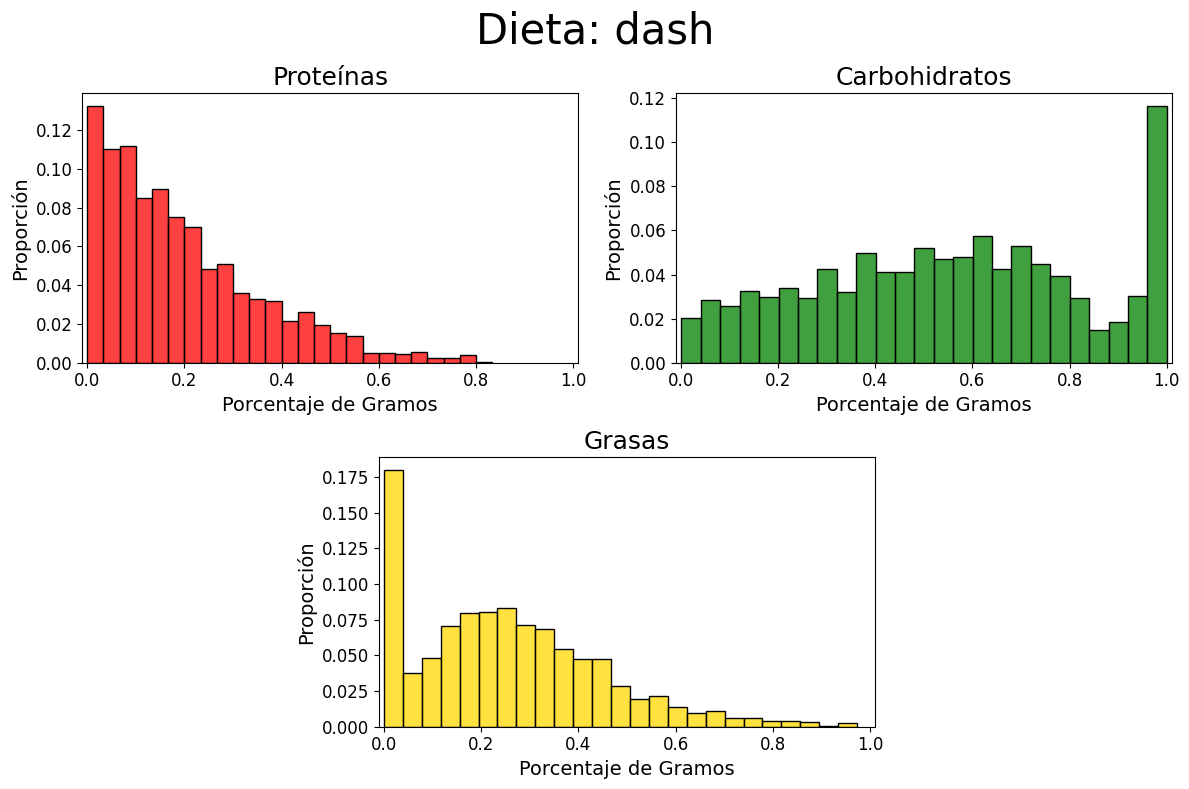
\includegraphics[width=0.75\textwidth]{Resources/2_03_plot_01.png}
            \end{center}

        \subsubsection{Dieta Keto}

            Una receta de esta dieta tendrá que, en promedio, el $50\%$ de 
            sus macronutrientes son grasas, esto se relaciona con el hecho de 
            que se intenta inducir la ketosis (principio en que se basa esta         
            dieta); el $30\%$ son proteínas, notando que se intenta reducir 
            el consumo de carbohidratos; y el $20\%$ son carbohidratos, 
            resaltando ser una dieta baja en carbohidratos.\\

            El cincuenta por ciento de las recetas tienen entre el $40\%$ y 
            $60\%$ de grasas en su composición, denotando que existe una alta 
            concentración de recetas con una alta composición en grasas. Y, de 
            igual manera, el cincuenta por ciento de las recetas tienen entre 
            el $8\%$ y $26\%$ de carbohidratos, verificándose el hecho de que 
            se quiere minimizar el consumo de carbohidratos.\\

            En las proteínas, se puede observar que es como un caso intermedio, 
            debido a que, usando su rango intercuartil, la distribución de valores 
            que toma es amplia pero sigue siendo valores menores a los que se puede 
            encontrar en grasas. Esto es consecuencia de que se quiere intentar 
            eliminar el consumo de carbohidratos mientras se incrementa el consumo 
            de grasas.

            \begin{center}
                \begin{tabular}{| c | c c c |}
                    \toprule
                    Medida & Carbs(g) & Protein(g) & Fat(g) \\
                    \midrule
                    Media               & 0.200879 & 0.301777 & 0.497344  \\
                    $Q_1$               & 0.085517 & 0.158284 & 0.405354  \\
                    $Q_2$               & 0.157348 & 0.302900 & 0.505751  \\
                    $Q_3$               & 0.267535 & 0.409453 & 0.591887  \\
                    Desviación Estándar & 0.160609 & 0.167027 & 0.166572  \\
                    Mínimo              & 0.002060 & 0.000000 & 0.000000  \\
                    Máximo              & 1.000000 & 0.856868 & 0.997940  \\
                    Asimetría de Fisher & 1.634945 & 0.314795 & -0.147406 \\
                    \bottomrule
                \end{tabular}
            \end{center}

            Como los tres macronutrientes reportan una desviación estándar similar, 
            se tiene que es indicio de que las recetas son similares en su composición 
            de macronutrientes, es decir, diferentes recetas reportan composiciones 
            semejantes pero que se conforman de distintos alimentos o productos.\\

            Como la proporciones de carbohidratos cuenta con un sesgo positivo, se 
            tiene que refuerza el hecho de ser una dieta baja en carbohidratos. 
            De los aportes de grasas, se observa que su sesgo es despreciable implicando 
            que existen recetas tanto con aportes altos de este macronutriente (lo que se 
            busca) mientras que hay recetas con una contribución baja o nula del mismo.
            
            \begin{center}
                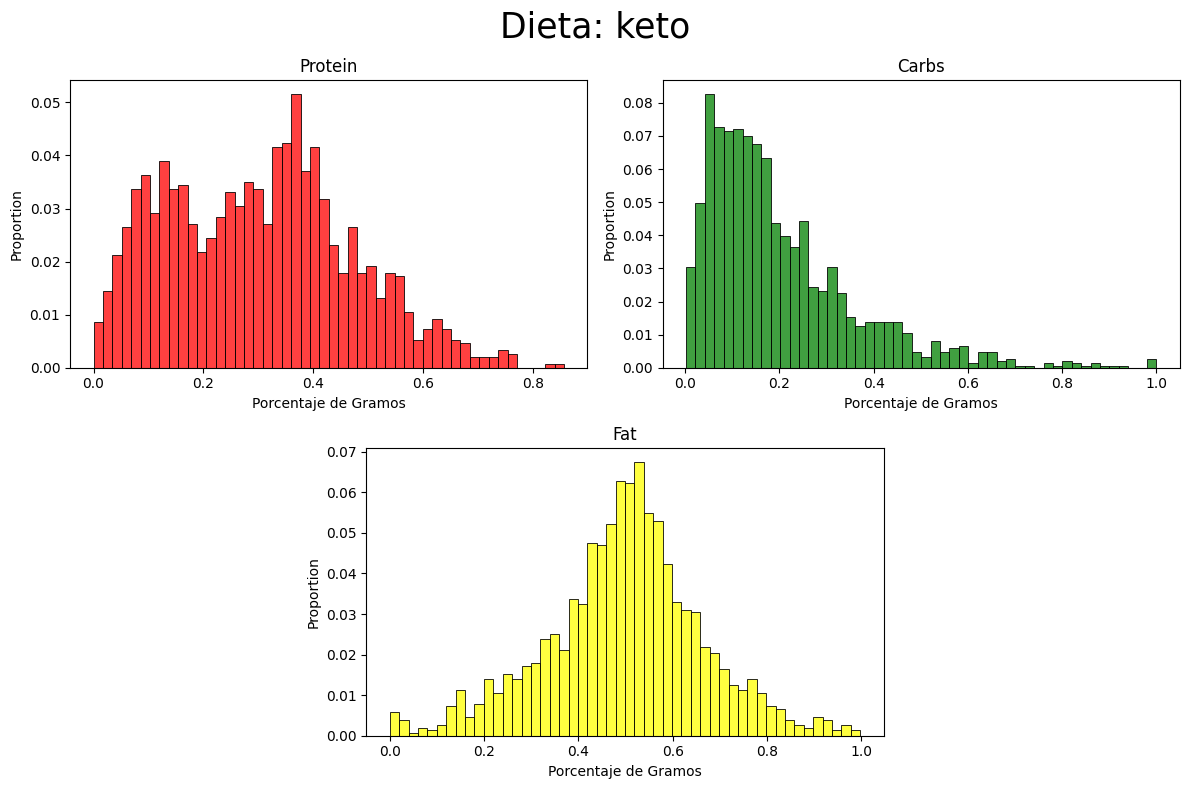
\includegraphics[width=0.75\textwidth]{Resources/2_03_plot_02.png}
            \end{center}

        \subsubsection{Dieta Mediterránea}

            Una receta de esta dieta tendrá que, en promedio, el $42\%$ de sus 
            macronutrientes son carbohidratos, esto debido a un alto consumo de 
            productos como, frutas, vegetales y granos enteros; el $30\%$ son 
            grasas, resaltando un alto consumo de nueces y aceite de oliva, como 
            también un consumo moderado de pescado; y el $28\%$ son proteínas, 
            vinculado con un consumo moderado de pescado y aves de corral, y un 
            bajo consumo de carnes rojas.\\

            El cincuenta por ciento de las recetas tienen entre el $25\%$ y $60\%$ 
            de carbohidratos en sus aportes, reflejando una alta variedad de composiciones 
            sobre este macronutriente. Esto debido a los alimentos base de esta dieta y 
            al valor reportada para su desviación estándar,haciendo posible esta 
            diversidad de valores.\\

            En el caso de las proteínas y grasas, muestras distribuciones que siguen 
            patrones similares en el sentido de que sus desviaciones estándar y rangos 
            intercuartiles son similares. Por lo que las recetas, por al menos en estos 
            macronutrientes, tienen composiciones similares. Específicamente, el cincuenta 
            por ciento de ellas tiene entre el $16\%$ y $38\%$ de proteínas	y el $18\%$ y 
            $39\%$ de grasas en la composiciones de estos macronutrientes.

            \begin{center}
                \begin{tabular}{| c | c c c |}
                    \toprule
                    Medida & Carbs(g) & Protein(g) & Fat(g) \\
                    \midrule
                    Media               & 0.424493 & 0.279357 & 0.296150  \\
                    $Q_1$               & 0.249955 & 0.159633 & 0.180357  \\
                    $Q_2$               & 0.439382 & 0.227883 & 0.268336  \\
                    $Q_3$               & 0.607531 & 0.377820 & 0.390404  \\
                    Desviación Estándar & 0.214325 & 0.162853 & 0.160783  \\
                    Mínimo              & 0.006733 & 0.005036 & 0.001731  \\
                    Máximo              & 0.992746 & 0.887557 & 0.968722  \\
                    Asimetría de Fisher & -0.096055 & 0.955922 & 0.869493 \\
                    \bottomrule
                \end{tabular}
            \end{center}

            La amplia variedad en la composición de macronutrientes en las recetas podría 
            estar relacionada con la internacionalización de esta dieta, en específico, de 
            tomar inspiración de recetas y adaptarlas a los productos disponibles en 
            ciertas regiones geográficas.\\

            La proporción de proteínas está segada positivamente y junto con una 
            alta acumulación de recetas con bajo porcentaje de proteínas, se tiene que 
            esta dieta figura como una con bajo consumo de alimentos ricos en proteínas. 
            
            \begin{center}
                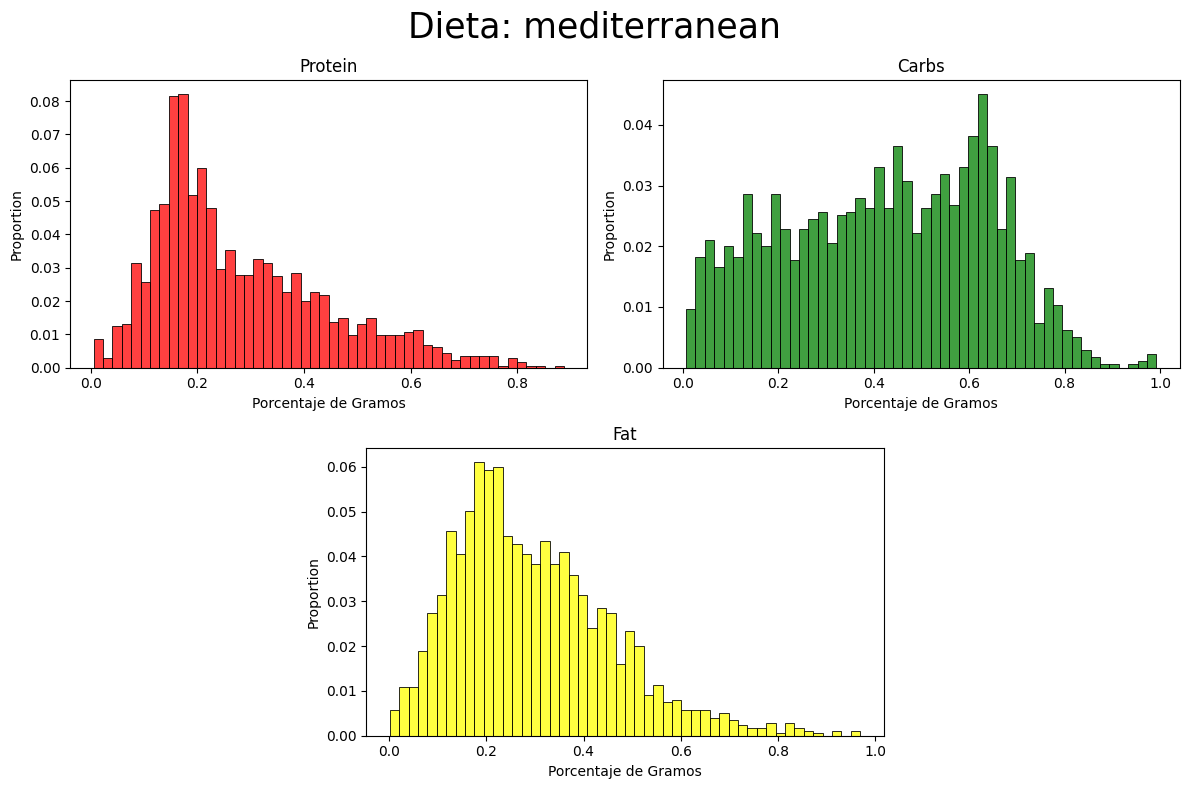
\includegraphics[width=0.75\textwidth]{Resources/2_03_plot_03.png}
            \end{center}

        \subsubsection{Dieta Paleo}

            Una receta de esta dieta tendrá que, en promedio, el $38\%$ de sus 
            macronutrientes son grasas y el $37\%$ son carbohidratos, esto se 
            relaciona con el consumo de productos como frutas, vegetales, nueces 
            y semillas; y el $25\%$ son proteínas cuyas principales fuentes son 
            carnes margas y pescado.\\

            El cincuenta por ciento de las recetas tienen entre el $19\%$ y $51\%$ 
            de carbohidratos en sus aportes, indicando una alta variedad de recetas 
            respecto a este macronutriente, esto se debe al consumo de alimentos que 
            se encuentran en la naturaleza o en estado salvaje (excluyendo algunos 
            de ellos).\\

            Como las proteínas y grasas tienen desviaciones estándar similares, refleja 
            que los alimentos y productos asociados a estos macronutrientes no tengan 
            una alta diversidad. Es decir, las recetas tienen muchos productos y alimentos 
            en común. En cambio, sus rangos intercuartiles difieren, mostrando como 
            las proteínas, sus valores, están más concentradas en un rango menor en 
            comparación con el de las grasas.

            \begin{center}
                \begin{tabular}{| c | c c c |}
                    \toprule
                    Medida & Carbs(g) & Protein(g) & Fat(g) \\
                    \midrule
                    Media               & 0.371307 & 0.249693 & 0.379000  \\
                    $Q_1$               & 0.192399 & 0.102963 & 0.256579  \\
                    $Q_2$               & 0.351300 & 0.205532 & 0.382447  \\
                    $Q_3$               & 0.515054 & 0.375392 & 0.488116  \\
                    Desviación Estándar & 0.221506 & 0.175031 & 0.175471  \\
                    Mínimo              & 0.003612 & 0.000000 & 0.001404  \\
                    Máximo              & 0.987368 & 0.858503 & 0.968835  \\
                    Asimetría de Fisher & 0.488656 & 0.711408 & 0.312673  \\
                    \bottomrule
                \end{tabular}
            \end{center}

            La posible limitante de alimentos asociados a proteínas	y grasas 
            podría impactar en que las recetas estén hechas con los mismos productos 
            dentro de la misma región geográfica. Estos se relacionaría con una 
            baja variedad en la presencia de estos macronutrientes.\\

            Se observa como las recetas tienden a tener una contribución moderada de 
            carbohidratos y grasas, esto se relaciona con los principales alimentos 
            que son consumidos en esta dieta. Mientras que sus aportes de proteínas 
            son bajas en comparación con los otros dos macronutrientes.
            
            \begin{center}
                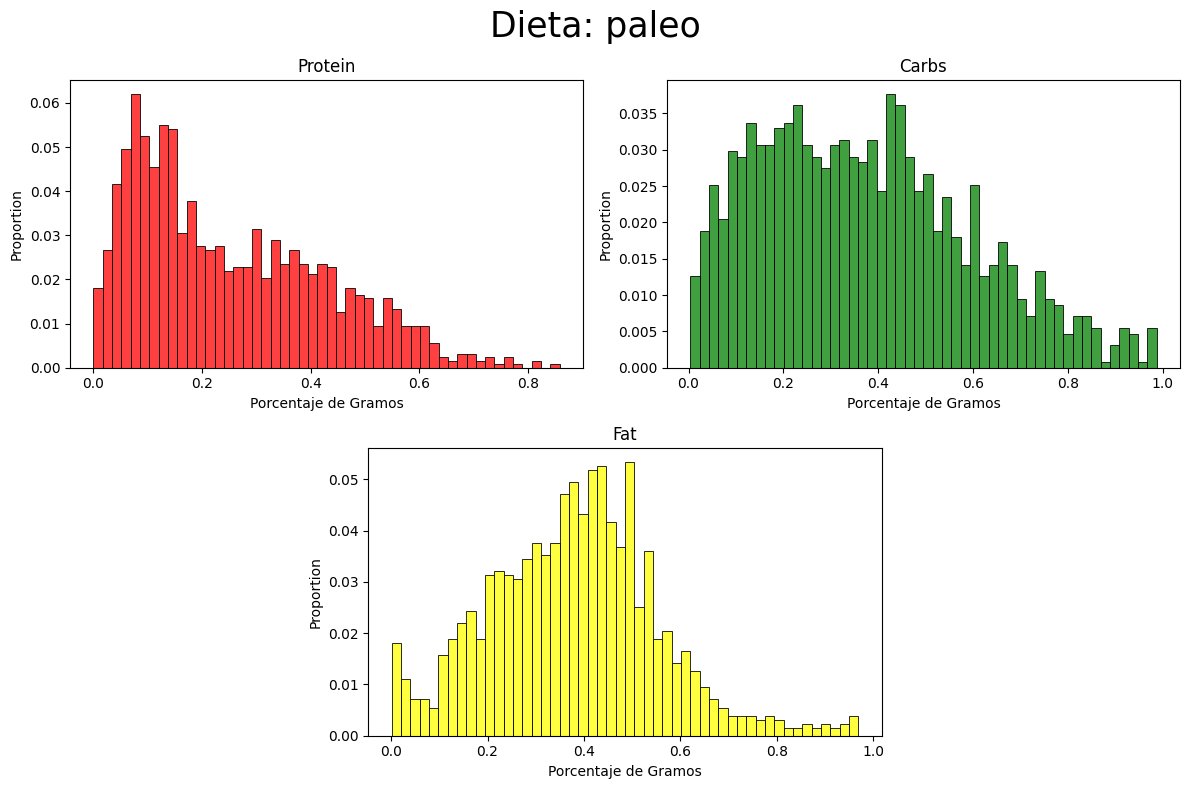
\includegraphics[width=0.75\textwidth]{Resources/2_03_plot_04.png}
            \end{center}

        \subsubsection{Dieta Vegana}

            Una receta de esta dieta tendrá que, en promedio, el $60\%$ de 
            sus macronutrientes son carbohidratos, que provienen de fuentes 
            como vegetales, frutas, cereales y legumbres; el $25\%$ son grasas, 
            relacionadas con el consumo de nueces y semillas; y el $15\%$ son 
            proteínas, esto debido a un nulo consumo de alimentos de origen 
            animal y que estas fuentes son reemplazadas por fuentes vegetales.\\

            El cincuenta por ciento de las recetas tienen entre el $50\%$ y el $71\%$ 
            de carbohidratos en su composición, esto debido al alto consumo de 
            alimentos ricos en carbohidratos en origen vegetal, los cuales son 
            muy diversos.\\

            Mientras que el cincuenta por ciento de las recetas tienen entre el $14\%$ y 
            el $34\%$ de grasas en su composición, esto se relaciona al hecho de que 
            existen alimentos de origen vegetal ricos en grasas no animales.\\
            
            En las proteínas, se puede observar un rango intercuartil reducido y una 
            desviación estándar reducida, esto evoca a que las recetas tengan bajos 
            aportes de proteínas así como también los valores de aportes se concentren 
            en un rango reducido. En específico, el cincuenta por ciento de las recetas 
            tienen entre el $8\%$ y el $19\%$ de proteínas.

            \begin{center}
                \begin{tabular}{|c|ccc|}
                    \hline
                    Medida & Carbs(g) & Protein(g) & Fat(g) \\
                    \hline
                    Media               & 0.593968 & 0.148489 & 0.257543  \\
                    $Q_1$               & 0.504070 & 0.085339 & 0.142575  \\
                    $Q_2$               & 0.626246 & 0.139688 & 0.231518  \\
                    $Q_3$               & 0.714679 & 0.190381 & 0.344529  \\
                    Desviación Estándar & 0.171203 & 0.086088 & 0.160277  \\
                    Mínimo              & 0.000330 & 0.001921 & 0.000112  \\
                    Máximo              & 0.986872 & 0.647416 & 0.994887  \\
                    Asimetría de Fisher & 0.189556 & 0.922401 & 0.461455  \\
                    \hline
                \end{tabular}
            \end{center}

            Debido a que los carbohidratos y grasas reportan desviaciones estándar 
            similares, sería indicio de que las recetas tienen composiciones similares 
            para estos dos macronutrientes.\\

            De las proporciones de proteínas, se resalta una alta acumulación de 
            recetas con bajos aportes de proteínas, esto hace de esta dieta una 
            con bajo consumo de proteínas. Lo último debido a que las principales 
            fuentes proteínas son animales y haciendo que los aportes de carbohidratos 
            sean altos en comparación con los otros dos macronutrientes.

            \begin{center}
                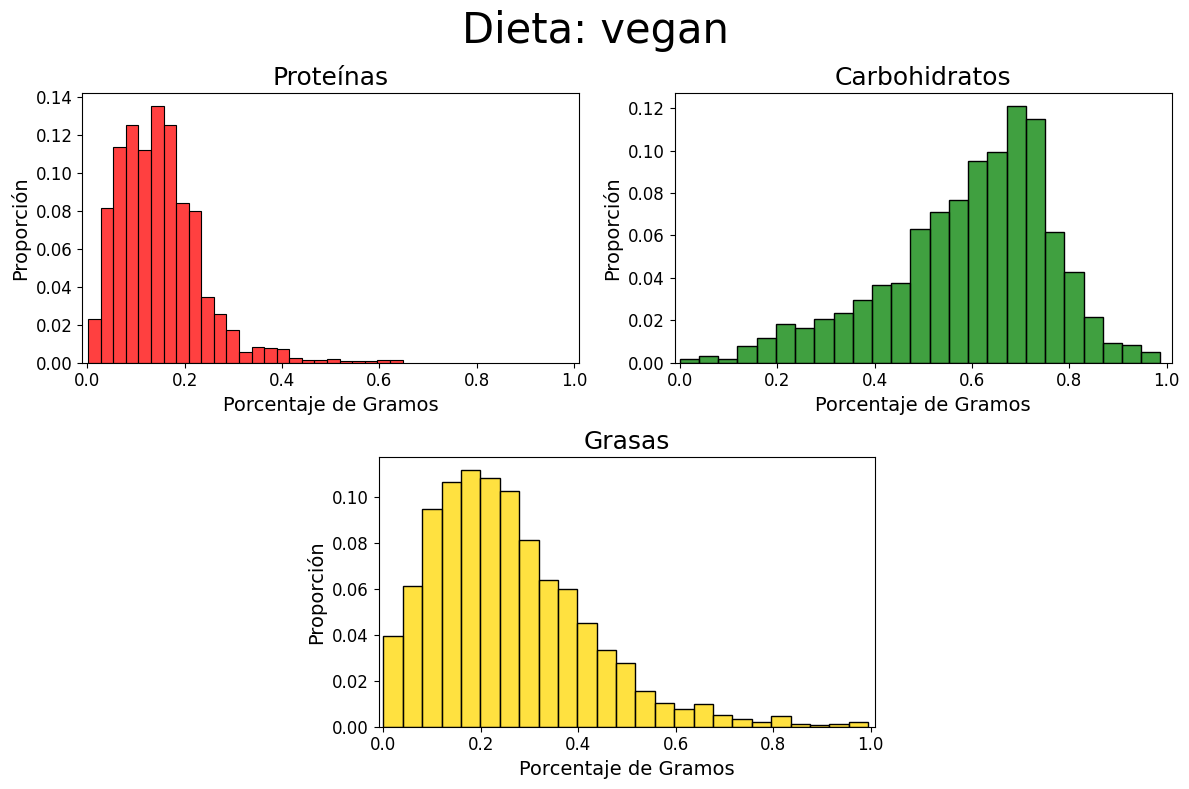
\includegraphics[width=0.75\textwidth]{Resources/2_03_plot_05.png}
            \end{center}

        \subsubsection{Gráfico de Cajas y Bigotes de la distribución de Macronutrientes por Dieta}
            Se anexan las gráficas de cajas y bigotes de las distribuciones de los 
            macronutrientes por dieta para apoyar las observaciones realizadas anteriormente. 
            Resaltando el comportamiento esperado en los macronutrientes por dieta que, junto 
            con el análisis dan paso a las reglas que se aplicarán para la eliminación de recetas 
            atípicas que presentan las diferentes dietas.

            \begin{center}
                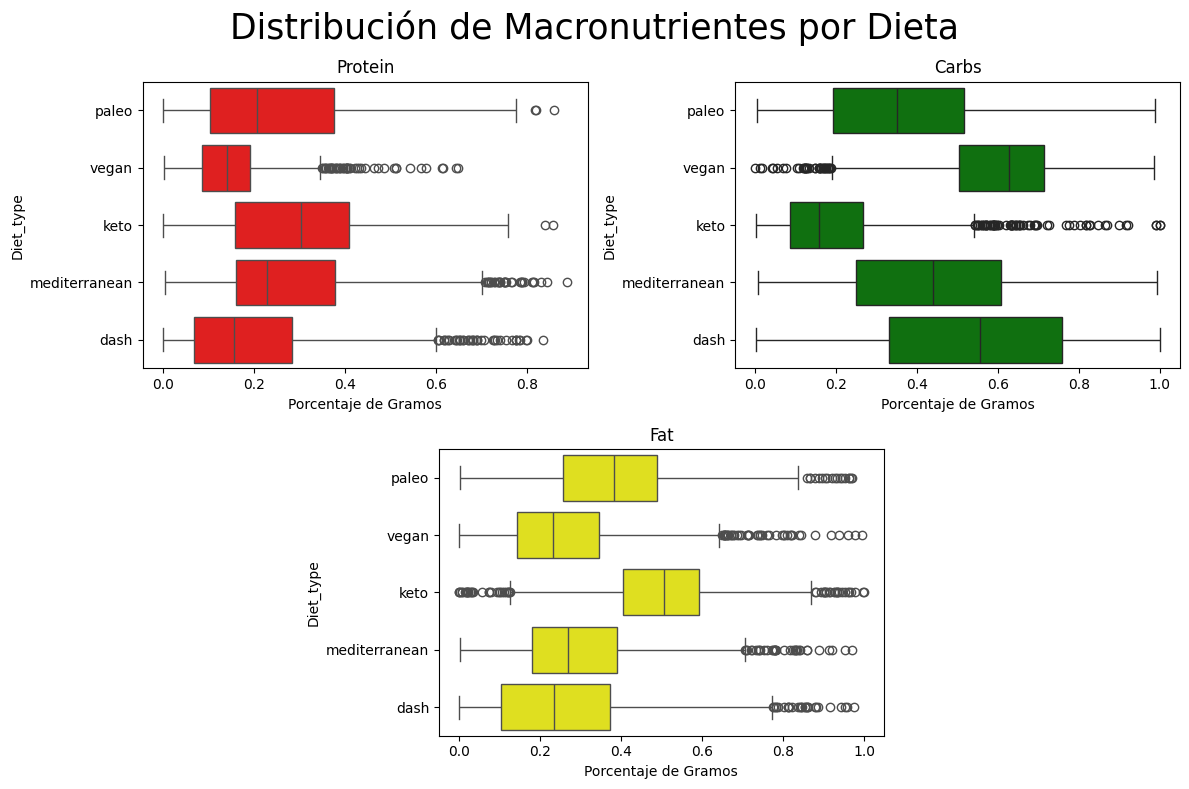
\includegraphics[width=0.75\textwidth]{Resources/2_03_plot_06.png}
            \end{center}

\newpage

\printbibliography[heading=bibintoc,title={Referencias Bibliográficas}]

\end{document}